%!TEX TS-program = xelatex
%!TEX encoding = UTF-8 Unicode

%\def \papersize {a4paper}
\def \papersize {letterpaper}
\documentclass[12pt,\papersize]{extarticle}
% extarticle is like article but can handle 8pt, 9pt, 10pt, 11pt, 12pt, 14pt, 17pt, and 20pt text

\def \ititle {Interacting Mindreaders}
\def \isubtitle {}
\def \iauthor {Stephen A. Butterfill}
\def \iemail{s.butterfill@warwick.ac.uk}
%\def \iauthor {}
%\def \iemail{}
\date{}


%!TEX TS-program = xelatex
%!TEX encoding = UTF-8 Unicode

\title{\ititle\\\isubtitle}
\author{\iauthor\\<{\iemail}>}

\usepackage[\papersize]{geometry} % see geometry.pdf
\geometry{twoside=false}
\geometry{headsep=2em} %keep running header away from text
\geometry{footskip=1cm} %keep page numbers away from text
\geometry{top=3cm} %increase to 3.5 if use header
\geometry{left=4cm} %increase to 3.5 if use header
\geometry{right=4cm} %increase to 3.5 if use header
\geometry{textheight=22cm}

%non-xelatex
%\usepackage[T1]{fontenc}
%\usepackage{tgpagella}

%for underline
\usepackage[normalem]{ulem}

%get the font here:
% http://scripts.sil.org/CharisSILfont

\usepackage{fontspec,xunicode}
%nb do not explicitly use package xltxtra because this introduces bugs with footnote superscripting  -- perhaps because fontspec is supposed to include it anyway.
%UPDATE:  "You need to use the no-sscript option in xltxtra: \usepackage[no-sscript]{xltxtra}, this is explained in the documentation of xltxtra.  The issue is that Sabon does not contain true superscript glyphs for every character and the no-sscript option will instead use scaled regular glyphs, which is typographically inferior, but there is no other option available when using Sabon." --- http://groups.google.com/group/comp.text.tex/browse_thread/thread/19de95be2daacade
\defaultfontfeatures{Mapping=tex-text}
%\setromanfont[Mapping=tex-text]{Charis SIL} %i.e. palatino
%\setromanfont[Mapping=tex-text]{Sabon LT Std} 
%\setromanfont[Mapping=tex-text]{Dante MT Std} 
%\setromanfont[Mapping=tex-text,Ligatures={Common}]{Hoefler Text} %comes with osx
\setromanfont[Mapping=tex-text]{Linux Libertine O} 
\setsansfont[Mapping=tex-text]{Linux Biolinum O} 
\setmonofont[Scale=MatchLowercase]{Andale Mono}


%hyperlinks and pdf metadata
%TODO avoid duplication of title & author
\usepackage{hyperref}
\hypersetup{pdfborder={0 0 0}}
\hypersetup{pdfauthor={\iauthor}}
\hypersetup{pdftitle={\ititle\isubtitle}}


%handles references to labels (e.g. sections) nicely
\usepackage{varioref}

%line spacing
\usepackage{setspace}
%\onehalfspacing
%\doublespacing
\singlespacing

\usepackage{natbib}
%\usepackage[longnamesfirst]{natbib}
\setcitestyle{aysep={}}  %philosophy style: no comma between author & year

%enable notes in right margin, defaults to ugly orange boxes TODO fix
%\usepackage[textwidth=5cm]{todonotes}

%for comments
\usepackage{verbatim}

%footnotes
\usepackage[hang]{footmisc}
\setlength{\footnotemargin}{1em}
\setlength{\footnotesep}{1em}
\footnotesep 2em

%tables
\usepackage{booktabs}
\usepackage{ctable}

%section headings
\usepackage[sf]{titlesec}
%\titlespacing*{\section}{0pt}{*3}{*0.5} %reduce vertical space after header
%large headings:
%\titleformat{\section}{\LARGE\sffamily}{\thesection.}{1em}{} 
\titlelabel{\thetitle.\quad}

%captions
\usepackage[font={small,sf}, margin=0.75cm]{caption}

%lists
\usepackage{enumitem}
\newenvironment{idescription}
{ 	
	% begin code
	\begin{description}[
		labelindent=1.5\parindent,
		leftmargin=2.5\parindent
	]
}
{ 
	%end code
	\end{description}
}


%title
\usepackage{titling}
\pretitle{
	\begin{center}
	\sffamily
	\Huge
} 
\posttitle{
	\par
	\end{center}
	\vskip 0.5em
} 
\preauthor{
	\begin{center}
	\normalsize
	\lineskip 0.5em
	\begin{tabular}[t]{c}
} 
\postauthor{
	\end{tabular}
	\par
	\end{center}
}
\predate{
	\begin{center}
	\normalsize
} 
\postdate{
	\par
	\end{center}
}


%\author{}

%\setromanfont[Mapping=tex-text]{Sabon LT Std} 

\begin{document}

\setlength\footnotesep{1em}

\bibliographystyle{newapa} %apalike


\tolerance=5000

\maketitle
%\tableofcontents

\begin{abstract}
\noindent
Could interacting mindreaders be in a position to know things which they would be unable to know if they were manifestly passive observers?  This paper argues that they could.  Mindreading is sometimes reciprocal: the mindreader's target reciprocates by taking the mindreader as a target for mindreading.  The paper explains how such reciprocity can significantly narrow the range of possible interpretations of behaviour where mindreaders are, or appear to be, in a position to interact.  A consequence is that revisions and extensions are needed to standard theories of the evidential basis of mindreading.  The view also has consequences for understanding how abilities to interact combined with comparatively simple forms of mindreading may explain the emergence, in evolution or development, of sophisticated forms of social cognition.

\

%\noindent
%Word count: 10 100

%
%What evidence grounds ascriptions of thoughts and actions,
%and how does the evidence support the ascriptions?
%In answering this question, 
%philosophers sometimes focus on mere observation, ignoring interaction.
%The only evidence considered is 
% evidence that would be available to mindreaders 
%observing their targets but in no position to interact with them.
%The present paper,
%which focuses on goal ascription,
%argues that this is a mistake
%and
%identifies evidence 
%available only to mindreaders capable of interacting with their targets.
%Being poised to interact with others may make it possible to know things about their thoughts and actions which one might not otherwise be in a position to know.
%This has consequences for the possible roles of interaction in explaining the evolution and development of mindreading. 
%
%What evidence grounds ascriptions of goals to other agents' actions,
%and how does the evidence support the ascriptions?
%It is usually assumed that, in answering this question, 
%we can focus on observation and ignore interaction.
%We can restrict ourselves to evidence that would be available to mindreaders who observe their targets but are not necessarily in a position to interact with them.
%The present paper identifies evidence 
%which supports goal ascriptions
%and 
%is available only to mindreaders who are capable of interacting with their targets.


\end{abstract}


\section{On the evidential basis of mindreading}
\label{sec:intro}

Mindreading is
the process of identifying thoughts and actions on the basis of bodily movements,
somewhat as reading is the process of identifying propositions on the basis of inscriptions \citep[p.\ 4]{Apperly:2010kx}.
Contrast
a mindreader who is, or appears to be, capable of interacting with her targets 
and
a mindreader who can manifestly only observe.
Is it possible that the interacting mindreader is in a position to know things which she would be unable to know if she were unable to interact with her targets?
Our aim in this paper is to argue that the answer is a qualified `yes'.

The question is about the evidential basis of mindreading, 
not about what sorts of mechanisms are involved.
While philosophers have engaged with questions about mechanisms (such as whether mindreading involves a process of simulation or of theorizing or some combination of the two),
comparatively little effort has recently been devoted to issues about what evidence could ground mindreading.

Our question is part of a broader question,
What is the evidential basis for ascriptions of thought and action and how does the evidence support the ascriptions?
%\footnote{
%See e.g.\ \citet[pp.\ 126-7]{Davidson:1973jx}.
%}
%To stress that this question is not directly about about \emph{how} anyone actually ascribes thoughts or identifies actions% 
%% nor directly about the mechanisms, processes or representations involved in mindreading
%, Davidson 
%sometimes formulates the question by asking what someone \emph{could} know that \emph{would} put them in a position to identify another's thoughts and actions.%
%\footnote{
%See, e.g., \citet[p.\ 126]{Davidson:1973jx}.
%While what follows draws  on Davidson's questions and insights,
%our aims here are more modest than his.
%For here we are concerned only with a  fraction of the problem of ascribing mental states and meanings,
%and we are not concerned with larger claims about mind, meaning and truth 
%(on which see 
%\citet{Davidson:1990du} and 
%\citet{lepore_donald_2005}).
%}
The most sustained attempts to answer this question,
Davidson's (\citeyear{Davidson:1984wh}; \citeyear{Davidson:1990du}), Lewis' (\citeyear{lewis:1974ri}) and Dennett's (\citeyear{Dennett:1987sf}),
do not exploit the possibility of interaction.
The evidence and principles they consider are available to manifestly passive observers.
So on their theories,
a purely passive mindreader observing from behind a one-way mirror
is on a par with
a mindreader who, actually or apparently, could interact with those she seeks to interpret.
The two are on a par in this sense:
in principle the same evidence could be available to each, and each can exploit the routes to knowledge in moving from evidence to ascriptions of thought and action.
Of course these theories are all compatible with the idea that interaction might be useful for mindreading in practice.  
But on these theories interaction makes no difference to what can in principle be known.
In this paper we aim to show
that mindreaders actually or apparently capable of interacting with their targets are at an advantage not only in practice but also in theory.
Their ascriptions could exploit routes to knowledge which would be unavailable if they were entirely passive observers.

Why suppose, in advance of considering the details, that interacting mindreaders might know more?
A mindreader's target is often also a mindreader and may sometimes reciprocate by taking the mindreader as a target for mindreading.
%Where this happens we have mindreaders mindreading and being mindread by mindreaders.
%The mindreader is her target's target for mindreading.
It ought to be possible, in mindreading, to make use of this reciprocity.
%of the fact that the mindreader's target reciprocates by taking the mindreader to be a target for mindreading.
But how could such reciprocity facilitate mindreading?
If we assume the mindreader is merely observing her target,
that there is manifestly no potential for interaction,
then it seems that any way of exploiting reciprocity would involve higher-order ascriptions. 
The mindreader would ascribe to her target beliefs (say) about the mindreader's own beliefs and other mental states.
And if her target reciprocates, she might escalate by ascribing to the target beliefs about her own beliefs about the target's beliefs about her beliefs.
While this might be useful in some situations, 
the nesting this approach requires quickly becomes dauntingly complex.
And the basic intuition about reciprocal mindreading goes unsatisfied.
Reciprocal mindreading should sometimes result in 
something like a meeting of minds
rather than
an escalation of higher-order ascriptions.
Perhaps fully exploiting reciprocity in mindreading
requires the mindreaders to be in a position to interact with each other;
perhaps in some cases 
being or appearing poised to interact
can somehow enable mindreaders to exploit reciprocity without first having to ascribe higher-order mental states.
This is the hunch we develop in what follows.


Even if the hunch turns out to be right, why investigate it?
One reason is that the investigation will enable us to revise and extend existing accounts of the evidential basis of mindreading  in ways that make them more accurate and comprehensive.
Another motive concerns the emergence, in evolution or in development, of mindreading.
Several researchers have offered quite general conjectures about how interaction might explain the emergence of sophisticated forms of cognition.
One view is that needs to interact with others have driven and shaped some aspects of cognition.%
\footnote{
E.g.\ \citet[p.\ 103]{Knoblich:2006bn} suggest that 
`functions traditionally considered hallmarks of individual cognition originated through the need to interact with others'
and that
`perception, action, and cognition are grounded in social interaction.'
}
We shall not speak to this view here.
Another view is that abilities to interact with others
may have fostered the emergence in evolution---or, on a different view, in development---%
of sophisticated forms of cognition including social cognition and, in particular, mindreading.%
\footnote{
\citet[p.\ 1]{Moll:2007gu}
argue for the `Vygotskian Intelligence Hypothesis' according to which `the unique aspects of human cognition ... were driven by, or even constituted by, social co-operation.'
See also
	\citet{Hughes:2004zj},
	\citet{Hughes:2006fu},
	\citet{Tomasello:2007gl} and
	\citet{tomasello:2008origins}.
}
Studying how interaction broadens the evidential basis of mindreading will eventually point to one way of filling in some details on just how interaction might facilitate the emergence of sophisticated forms of mindreading.

Our claim needs to be qualified in several ways.
First, we should highlight something already explicit but not yet emphasised:
the claim applies not just to 
 mindreaders who actually could interact with their targets
but also to
 mindreaders who appear to their targets to be potential interaction partners (even if they are not).
Trading the risk of a minor misunderstanding for concision we use the term `interacting mindreader' to refer to both groups;
similarly, references to mindreaders who `only observe' must be understood as excluding those who appear to their targets to be interaction partners.
Only cases involving the first group---mindreaders who actually could interact---are likely to be of wider interest.
%Cases involving misleading appearances might be regarded as artefacts of the model.
Any application of our claim to understanding evolution or development is bound to focus on cases where mindreaders actually could interact with their targets.

A second qualification concerns the scope of mindreading.
In most discussions of mindreading, the focus is on  ascription of beliefs and other mental states to individuals.
But in what follows we shall focus on the ascription of goals to actions.
Some might claim that goal ascription is not mindreading, perhaps because 
identifying relations between actions and the outcomes to which they are directed
does not necessarily involve ascribing mental states.
Our view is consistent with this claim (and with its negation).
\label{goal_ascription_verify}
Evidence for ascriptions of belief and of other mental states often includes the occurrence (and non-occurrence) of goal-directed actions.
Identifying these actions typically requires goal ascription.
In some cases, then, 
evidence for the ascription of a goal
will indirectly support the ascription of a belief or other mental state---%
the evidence will support  a goal ascription which will in turn support the ascription of a belief (say) to the agent of the action.
Accordingly, even those who deny that goal ascription is mindreading should agree that sometimes evidence for goal ascription is indirectly evidence for ascription of belief and other mental states.
So whether or not goal ascription is deemed to be mindreading,
an individual's access to evidence for mindreading  depends in part on her access to evidence for goal ascription.
Our plan is to show that interacting mindreaders could exploit routes to knowledge of the goals of others' actions which are not available to mere observers.
In doing this we will be showing that
mindreaders poised to interact with others 
could know things about their minds 
which they might not otherwise be in a position to know.

%Because the leading theories have supposed that being able to interact makes no difference,
%they have treated the evidential basis for mindreading as more narrow than it truly is.
%This matters
%because broadening the evidential basis will enable us to give a more accurate and comprehensive theory of mindreading.
%And, as we shall argue, this in turn matters because it may bear on the possibility of explaining the emergence, in evolution or in development, of mindreading.

Developing these ideas requires us to fill in some background on goal ascription and its limits, as well as on notions of goal-directed interaction.
Readers impatient to get to the central idea might skip to section \vref{sec:your_goal_is_my_goal}.



\section{Goal ascription}
Purposive action is action directed to the realisation of one or more outcomes.
Goal ascription is the process of identifying to which outcomes others' purposive actions are directed.
To illustrate, suppose that
Hannah kicks a ball thereby both preventing her sisters from scoring and also breaking a window.
Asked about the episode,
Hannah might protest, truthfully, that the goal of her action was not to break the window but only to reverse the others' advance.
As this illustrates,
among the actual and possible outcomes of an action,
only some are outcomes to which the action is directed.
Goal ascription is the process of identifying 
 those outcomes.
%, among an action's actual and possible outcomes,
%those to which it is directed.
%Our immediate question is therefore, 
%What evidence could support hypotheses about the outcomes to which actions are directed, 
%and how would the evidence support the hypotheses?

We focus on goal ascription 
partly because this simplifies our argument,
but mainly because goal ascription is widely thought to be among the very earliest components of mindreading to emerge (or, if goal ascription is not mindreading, then it is a late precursor).%
\footnote{
See, for example,
\citet{Gergely:1995sq} and 
\citet{Woodward:1998dm}.
See also
\citet[p.\ 111, Box 1]{Baillargeon:gx}
on two subsystems
and 
\citet{Povinelli:2001jf} on `behavioural regularities' whose specification sometimes appears to involve goal-directed action.
}
By showing that
  interacting mindreaders may have access to 
  evidence for goal ascriptions 
  which is unavailable to those who merely observe,
we will eventually be able to indicate ways in which interaction could facilitate the emergence, in evolution or development, of more sophisticated forms of mindreading.%
\footnote{
There are various ways of understanding the idea that mindreading may come in several forms, some less conceptually or cognitively demanding than others.
For a range of views, see
 \citet{Apperly:2009ju},
 \citet{Call:2005qe},
 \citet{Doherty:2006wz},
 \citet{ONeill:2005ff}
 and
 \citet{Wellman:2001if}.
}

Because goal ascription has received little attention,
in this section
we shall 
briefly review some potential benefits of being able to identify goals
and then 
consider what sort of evidence might support goal ascription.

It is a familiar idea that goal ascription enables one to learn from others' successes.
For example,
if you know or can guess that another agent's actions are directed to opening a nut,
you may then be in a position to infer that the unfamiliar pattern of actions she is performing constitute a means to open nuts.
%\citep{Horner:2005pj}
%In a different case, knowing the goal of another agent's actions may enable you to discover a new use for a tool.
A slightly less familiar idea is that goal ascription enables one to learn from others' failures as well as their successes.
For example, suppose that while you are searching for some peanuts 
another agent attempts but fails to reach for a closed container.
In some circumstances,
if you know that the goal of the agent's action was to obtain the peanuts
then you now have evidence as to where they might be.\footnote{
\citet{hare_chimpanzees_2004} exploit this fact in testing chimpanzees' abilities to ascribe goals.
}
This is one illustration of how goal ascription could in principle enable us to learn from others' failures 
(\citealp{Want:2001hp} offer another).


Goal ascription enables one
to predict and manipulate others' actions.
If you know that an agent is engaged in a sequence of actions whose eventual goal involves retrieving some object,
you may be able to predict that the agent will go to where the object is at some point.\footnote{
For an application see \citet{Hare:2001ph}.
}
Equally, in some cases knowing this much about the goal of another's actions many enable you to assist them,
either 
by retrieving the object for them 
or else
by revealing the object's location to them.%
\footnote{
For a paradigm involving the former see \citet{warneken:2007sa};
on the latter, see \citet{Liszkowski:2008al}.
}

Goal ascription is also instrumental for ascribing propositional attitudes.
We have already mentioned 
   (\vpageref*{goal_ascription_verify})
that such ascriptions often involve 
confirming predictions about actions 
which in turn typically requires
identifying the goals of those actions.
In addition,
knowing which outcomes an action is directed to may constrain hypotheses about what an agent intends 
as well as
potentially providing information concerning what the agent knows, believes or desires.
For example,
if we know that the goal of an agent's action is to retrieve some peanuts,
and if we also know where all the peanuts are,
we may be able to infer that she does not know where the peanuts are,
or that she falsely believes that some of the peanuts are over there.%
\footnote{
\citet{Wimmer:1998kx} exploit this possibility in testing children's abilities to ascribe false beliefs.
}
(Of course this can also work the other way:
information about an agent's beliefs or other mental states may support conclusions about her goals.
Belief- and goal-ascriptions are mutually constraining.)

Now that we have reviewed some of the benefits goal ascription can bring,
what evidence could support ascriptions of goals to actions?
Consider the claim that 
knowledgeably identifying the goals to which actions are directed
depends on 
knowledge of the agents' intentions
which in turn depends 
on knowledge of their beliefs, desires and other mental states.
If this claim were true,
it would make no sense to discuss the evidential basis of goal ascription except in discussing the evidential basis of mindreading more generally.
However,
the falsity of this claim  is presupposed  in both developmental and comparative research on goal ascription.%
\footnote{ 
Compare \citet{Gergely:1995sq},
	\citet{Woodward:1998dm} and
	\citet{Penn:2007ey}
among many others.
}
And we know of no compelling reason for taking this claim to be true.
After all,
it is consistent with rejecting the claim to recognize that
 ascriptions of goals to actions
 constrain, and are constrained by,
 ascriptions of intentions and other mental states.
The existence of such constraints does not show that one could 
not know something about the goals of actions 
while  knowing nothing about the agents' mental states.
Further,
there do seem to be situations where knowledge of agents' goals does not require any knowledge of their mental states.
For instance,
suppose that two people are sitting opposite each other at a low table
 which is 
sparsely populated with objects.
The objects are all out in the open; manifestly, both can clearly see them.
If one person reaches to grasp one of these objects (the duck, say), 
must the other ascribe beliefs or other mental states in order to knowledgeably identify the goal of her action as that of grasping the duck?
On the face of it, she need not.  
Even if she had no ability to ascribe mental states, it seems she might nevertheless be in a position to identify the goal of the other's action.

While not decisive,
these considerations are perhaps sufficient to motivate 
exploring what evidence might support goal ascription.
According to 
what Csibra and Gergely call `the principle of rational action',
%
\begin{quote}
`an action can be explained by a goal state if, and only if, it is seen as the most justifiable action towards that goal state that is available within the constraints of reality.'%
\footnote{
\citet[p.\ 255]{Csibra:1998cx}; cf.\ \citet{Csibra:2003jv}.
A related but different `principle of efficiency' has been formulated by \citet[p.\ 1061]{Southgate:2008el}:
`goal attribution requires that agents expend the least possible amount of energy within their motor constraints to achieve a certain end.'
}
\end{quote}
%
Taking this idea as a rough starting point,
we propose that
%goal ascription could sometimes involve 
%identifying which potentially desirable outcomes 
%an observed action is the best available means to achieving.
%More carefully, our proposal is that 
these facts:
%
\begin{enumerate}
%
\item action $a$ is directed to some goal;
%
\item actions of $a$'s type are normally capable of being means of realising outcomes of $G$'s type in situations with the salient (to any concerned) features of this situation;
% 
\item no alternative type of action is both 
typically available to agents of this type 
and also 
such that actions of this type would be normally be significantly better\footnotemark \ means of realising outcome $G$ in situations with the salient features of this situation;
\footnotetext{
An action of type $a'$ is a better means of realising outcome $G$ in a given situation than an action of type $a$ if, for instance, actions of type $a'$ normally involve less effort than actions of type $a$ 
in situations with the salient features of this situation 
and everything else is equal; 
or if, for example, actions of type $a'$ are normally more likely to realise outcome $G$ than actions of type $a$
in situations with the salient features of this situation 
and everything else is equal.
}
%
\item the occurrence of outcome $G$ is typically desirable for agents of this type;
%
\end{enumerate}
%
and
%
\begin{enumerate}[resume]
\item there is no other outcome, $G'$, 
the occurrence of which would be at least comparably desirable for agents of this type 
and where (2) and (3) both hold of $G'$ and $a$
%
%where
%	the occurrence of $G'$ would be at least comparably desirable for agents of this type 
%%where
%%	$G$'s occurrence is not a means to $G'$'s nor conversely,
%and
%where  
%	(2) and (3) both hold of $G'$ and $a$
\end{enumerate}
%
may jointly constitute defeasible evidence for the conclusion that:
%
\begin{enumerate}[resume]
\item $G$ is a goal to which action $a$ is directed.
\end{enumerate}
%
We suggest that the above inference, from (1)-(5) to (6), is a route to knowledge of the goals of actions in this sense:
in some cases
it would be possible to know the premises without already knowing the conclusion;
and, 
in some of those cases,
knowing the premises could put one in a position to know the conclusion.%
\footnote{
Knowledge of the conclusion may not require explicit knowledge of 
	what is salient to others,
	what is desirable to them,
	or what makes actions better for them.
It is arguably sufficient that
the individual ascribing a goal 
is entitled to 
rely on being sufficiently similar to the target of her ascription 
with respect to 
these things.
%	what makes one action a better or worse means of realising an outcome than another action for her,  
%	what is desirable to her,
%	and what is salient to her.
}

Why accept this?
Suppose that 
	(1)-(5) are facts 
and that
	$G$ is not a goal to which action $a$ is directed.
Then from (1) we know that $a$ has a goal, call it $G'$.
And from (5) we can infer that either 
(i) 
the action, $a$, was not of a type that is normally capable 
of being a means to the outcome to which it was directed,
or
(ii) 
a significantly better (for instance, a more reliable or less effortful) means of achieving $G'$ is typically available to agents of this type,
or
(iii)
$G'$'s occurrence would be significantly less desirable than $G$'s occurrence for agents of this type.
So the agent's action fell short of being appropriate or optimal in some way,
or the agent has atypical preferences or capabilities,
or the situation is not normal.
While any of these is possible---%
and perhaps in some cases even to be expected---%
there are also circumstances in which it is reasonable to suppose that none obtains,
that the situation will be normal in relevant respects,
that agents will have typical preferences and capabilities 
and that they will act in ways that are appropriate and (in the limited sense in play here) optimal.
In such circumstances, the above inference can serve as a route to knowledge of the goals of actions.
The existence of this route to knowledge shows that goal ascription doesn't invariably depend on mental state ascription.

Note that we are not suggesting that the above inference captures the only route to knowledge of the goals of actions,
or that it provides anything like a comprehensive theory of the evidential basis of goal ascription.
Clearly it does not.
The inference has only limited applications.
For example, it cannot be used when an action is the best available means of achieving two or more comparably desirable outcomes. 
Fortunately the argument that follows does not depend on having a comprehensive theory of evidence for goal ascription.
The point of this brief discussion was only to 
consider the sort of evidence that can bear on goal ascription
and to 
show that 
even those incapable of ascribing mental states like belief 
might nevertheless have evidence sufficient for goal ascription.

Our narrow aim in what follows is to show that some routes to knowledge of the goals of actions 
are available only to interacting mindreaders
and not to those who merely observe.
Having in this section introduced goal ascription as a topic,
the next step is to identify an obstacle to acquiring knowledge of the goals of actions,
one which we will eventually show can be avoided where mindreaders can (or appear able to) interact with their targets.


\section{The problem of opaque means}
\label{sec:opaque_means}

While we lack a detailed theory of the evidential basis of goal ascription,
it is certain that the evidence for goal ascription sometimes includes considerations about which ends actions are means to.
Suppose an observer faces an action but cannot identify ends to which it could be a means.
This may prevent her from recognizing the action's goal%
\footnote{
It is possible that some actions have more than one goal.
To reduce parenthetical qualifications we shall write as if actions had only one goal.  
All of our key claims and arguments are consistent with the possibility of actions with more than one goal.
} 
 by depriving her of evidence.
To illustrate, contrast two cases of tool use.
In one case, someone uses a reamer to  juice  a lime; in the other, someone else scores shag with a lame to prevent a loaf from cracking.
Without communication, repetition or convention,
an observer familiar with reamers but not lames 
may be able to identify the goal of the first action only.
As this illustrates, ignorance about to which ends actions are means can be an obstacle to goal ascription.
Call this the problem of opaque means.

We are not suggesting that no observer could ever identify the goal of any action she fails to recognise as a means to achieving that goal.
Of course opaque means are not in every case an insurmountable obstacle to goal ascription, and
they may only rarely be a problem for human adults with sophisticated social skills.
Our point is neither novel nor surprising:
opaque means sometimes  deprive mindreaders of evidence and so prevent goal ascription.
This is more likely to happen where  goal ascribers lack sophistication in mindreading, communication and culture.

Some of the most plausibly unique aspects of human cognition depend on our abilities to recognise the goals of novel behaviours involving tools, and of communicative gestures.
The problem of opaque means is likely to arise in both cases
if goal ascription is based  entirely on observation 
(so that the possibility of interaction is ignored)
and if the goal ascriber lacks sophisticated social skills.
We have just seen an illustration of how the problem of opaque means arises where tools are used to unfamiliar ends.
Relatedly, it is also likely to arise where actions involve multiple steps that do not form a familiar sequence, can occur in various orders and can be interspersed among other activities;
as in preparing spirit from grain, for example.
%\footnote{
%*cut because 'plausibly unique aspects of human cognition'*
%one example is food preparation in some groups of mountain gorillas
%\citep[p.\ 531]{Byrne:2003wx}.
%*This is slightly tricky because Byrne wants a pure behaviour reading account with no understanding of intention.  
%Stress that this is consistent with supposing that goals are ascribed.
%}

The problem of opaque means also affects communicative actions 
 because these characteristically have  goals which the actions are means to realising only because others recognise them as means to realising those goals (a Gricean circle). 
To illustrate, consider an experiment from 
\citet[][experiment 3]{hare_chimpanzees_2004}
 whose two main conditions are depicted in figure \vref{fig:reach_point}.
The pictures in the figure stand for what participants, who were chimpanzees, saw.
The question was whether participants would be able to work out which of two containers concealed a reward.
In the condition depicted in the left panel, participants saw a chimpanzee trying but failing to reach for the correct container. 
Participants had no problem getting the reward in this case, suggesting that they understood the goal of the failed reach.
In the condition depicted in the right panel, a human pointed at the correct container.
Participants did not reliably  get the reward in this case, suggesting that they failed to understand the goal of the pointing action.%
\footnote{
The contrast between the two conditions is not due merely to the fact that one involves a human and the other a chimpanzee.
Participants were also successful when the failed reach was executed by a human rather than another chimpanzee \citep[][experiment 1]{hare_chimpanzees_2004}. 
}
This may be because of the problem of opaque means.
One theoretically possible explanation of these findings is that the participants could identify to which end a failed reach might be a means, but not to which end a communicative gesture might be a means.%
\footnote{
  \label{fn:communicative_intention}
Hare and Tomasello 
consider several explanations for their findings including `the hypothesis that chimpanzees do not understand the communicative intent of a cooperative-communicative experimenter' (\citeyear[p.\ 580]{hare_chimpanzees_2004}).
\citet[pp.\ 5--7]{Moll:2007gu} argue for a hypothesis along these lines by appeal to a range of related findings.
}
Whatever the truth about the chimpanzees' performance,
this possibility illustrates how the problem of opaque means can be an obstacle to exploiting communicative gestures.

\begin{figure}
\begin{center}
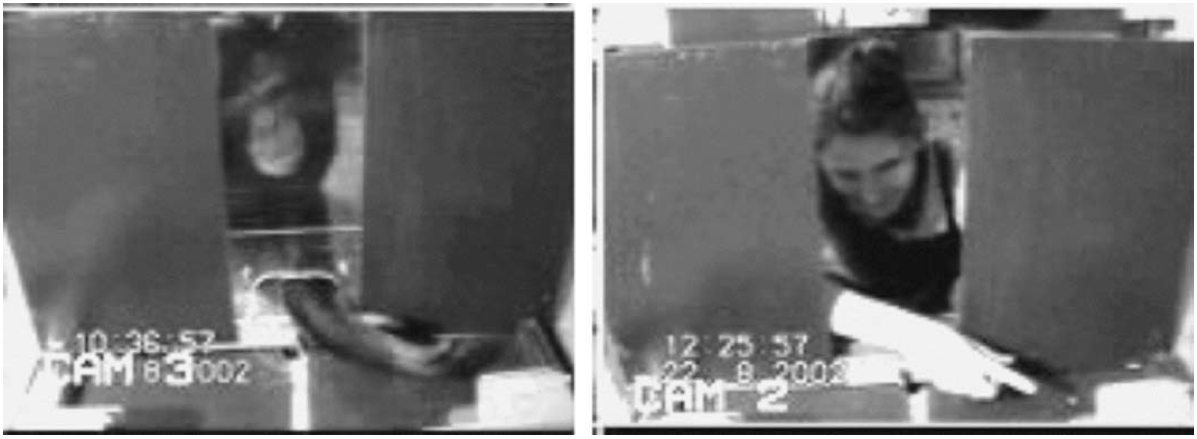
\includegraphics[width=12cm]{figure_hare_toma_2004_e3.png}
\caption{
\label{fig:reach_point}
	A failed reach (left) and a helpful point (right).
	Reproduced from \citet[p.\ 557, figure 4]{hare_chimpanzees_2004}.
}
\end{center}
\end{figure}

This, then, is the problem of opaque means:
failures to identify to which ends actions are means can impair goal ascription.
The problem is potentially a problem for mindreaders given the standard, purely observational theories of mindreading.
Note that it is not our intention to suggest that the problem of opaque means is a problem \emph{for theories of mindreading};
what matters for our purposes is only that it is a potential problem \emph{for mindreaders}.

That the problem of opaque means exists
is the first step in our argument
that 
theories of the evidential basis of mindreading based on pure observation 
are less powerful than theories taking into account the possibility of interaction.
They are less powerful in this sense: 
some routes to knowledge of the goals of actions are available only where a theory of the evidential basis of mindreading 
 takes the possibility of interaction into account.
In what follows we shall explain how being able to interact with another sometimes makes available a route to knowledge of the goals of her actions  which avoids the problem of opaque means.
This will support our claim that an interacting mindreader might be in a position to know things which she would be unable to know if she were only observing.


\section{Interactions involving distributive goals}
\label{sec:joint_action}
We aim eventually is to defend this claim:
there are routes to knowledge of the goals of others' actions
which are closed to
mindreaders who merely observe their targets
but open to 
mindreaders who are, or appear to be, capable of interacting with their targets.
As a preliminary to defending this claim,
we need to specify which types of interaction are relevant.
That is the aim of this section.

Let us stipulate that an outcome is a \emph{distributive goal} of two or more agents' actions just if two conditions are met.
\label{df:distributive_goal}
First, this outcome is  one to which each agent's actions are individually directed.
Second, each agent's actions are related to the outcome in such a way that it is possible for all the agents (not just any agent, all of them together) to succeed in bringing about this outcome.

To illustrate,
suppose that, while doing some gardening,
we find a turnip too big for any of us to easily pull out of the ground alone.
We each individually intend that we all pull up the enormous turnip
and we act on this intention.%
\footnote{
For an argument that it is possible for each of us individually to intend that we do something, see \citet{Bratman:1999fr} and \citet{Bratman:2012fk}.
}
There is a single outcome,
freeing the turnip,
to which each of our actions is individually directed.
And it is possible for all of us to succeed in bringing about this outcome.
So this outcome is a distributive goal of our actions.

%Contrast this episode with an alternative where no distributive goal is involved.
%Instead of intending that we all pull up the enormous turnip,
%each of us intends that she herself pull it up.
%While all of our actions are directed to similar outcomes (they all involve pulling up the turnip),
%these are clearly different outcomes.
%They are clearly different because one could occur while another did not;
%one of us might have broken an arm and been unable to pull while the others succeeded.
%So in this case, freeing the turnip is not a distributive goal of our actions.
%For some actions to have a distributive goal,
%it is necessary that there be a single outcome (and not merely similar outcomes) to which they are directed.

Note that our actions could have a distributive goal even without us each intending that we do something.
As another variation on the turnip-pulling story,
suppose that we each individually intend to 
	contribute to pulling up the turnip or pull it up.
Such intentions are agent neutral in this sense:
relative to such an intention an agent 
	could succeed by acting alone 
and
  she also could succeed by acting with unspecified other agents.
Plausibly our having these intentions is sufficient for our actions to have a distributive goal.
For in virtue of these intentions each of our actions is directed to the turnip's extraction,
and this is an outcome relative to which it is possible that all of our actions succeed.


In defining `distributive goal' we stipulated that it must be possible for all of the agents of actions with a distributive goal to succeed relative to that outcome.
Consider a variation on our first turnip-pulling story.
Instead of each intending that we pull up the turnip,
we each simply intend  to pull up the turnip.
In this case,
some might claim that
this amounts to us each intending that he or she pulls up the turnip.
And this claim might be taken to support the further claim that
there is no outcome to which each of our actions are directed
in virtue of our having these intentions
such that we could all succeed relative to this outcome.
%, given our intentions in this alternative case, we could not all succeed relative to the outcome of pulling up the turnip---%
%that if your actions were to succeed relative to the turnip's extraction,
%then ours would fail.
We take no stand on whether either claim is correct.
For our purposes all that matters is that there are distributive goals.
And the existence of distributive goals follows from the possibility of each of us 
intending that we pull up the turnip
(rather than simply
intending to pull it up),
and from the possibility of each of us
intending to contribute to pulling up the turnip or pull it up.

For two agents' actions to have a distributive goal it is sufficient that their actions constitute a joint action 
(at least this is true on almost any account of joint action).%
\footnote{
\label{fn:joint_action_distributive_goal}
We know of two definitions of joint action on which it is not straightforward that all joint actions involve distributive goals.
One is provided 
 is provided by \citet[p.\ 366]{ludwig_collective_2007} and quoted in footnote \vref{fn:ludwig}; the other is due to 
\citet[p.\ 70]{Sebanz:2006yq}.
According to Sebanz and colleagues' `working definition', 
`joint action can be regarded as any form of social interaction whereby two or more individuals coordinate their actions in space and time to bring about a change in the environment'
(\citeyear[p.\ 70]{Sebanz:2006yq}).
On one way of reading this, the latter part is equivalent to `a change in the environment is such that: to bring it about two or more individuals coordinate their actions';
 this does suggest that the actions have a distributive goal.
On other standard accounts it is straightforward that joint action involves distributive goals.
Compare 
	\citet[pp.\ 329-31]{Bratman:1992mi},
	\citet[pp.\ 96-7]{Searle:1990em} and
	\citet[pp.\ 168-9]{gilbert:2009shared}.
}
However, the converse does not hold.
As the first variation of the turnip-pulling story indicates,
two or more agents' actions may have a distributive goal 
even though the agents do not know about each others' intentions or actions.
In fact our actions might have a distributive goal even though none of us is aware of this, or even of the others' existence. 
(We resist the temptation to contrive a truly gigantic turnip and a pitch dark, very stormy night; readers can probably guess how this would go.)
One consequence of this is that 
two or more agents' actions may have a distributive goal
even though they are not engaged in joint action
(at least not on any standard account of joint action).%
\footnote{
On many accounts of joint action, each agent involved in a joint action must believe, expect or know something about the jointness of her action.
See 
	\citet[p.\ 103]{Bratman:1993je}, %common knowledge
	\citet[p.\ 40]{Butterfill:2011fk},
	\citet[p.\ 10]{Kutz:2000si}, %Agents acting on a shared intention have `a conception of themselves as contributors to a collective end.'
	\citet[p. 56]{miller_social_2001} % requires that each agent believes her actions are interdependent with the other agent's.
	and
	\citet[p.\ 361]{Roth:2004ki}. %: `each participant ... can answer the question of what he is doing or will be doing by saying for example ``We are walking together'' or ``We will/intend to walk together.''' 
Exceptions include  \citet{pacherie_framing_2011} and \citet{ludwig_collective_2007}.
\label{fn:ludwig}
According to Ludwig,
`The concept of a joint action as such is just that of an event of which there are multiple agents' (\citeyear[p.\ 366]{ludwig_collective_2007}).
Depending on what events are and what it is to be the agent of an event,
it may turn out that,
on Ludwig's definition,
our actions' having a distributive goal 
is sufficient for
us to be engaged in joint action.
}


The notion of a distributive goal is a 
narrowly technical one.
In introducing this notion by stipulation we are not aiming to match anyone's intuitions about anything.
What matters for now is just that the definition is theoretically coherent and that it is possible for actions to have distributive goals.
Our aim in introducing distributive goals 
 is to capture a minimal requirement on the sort of interactions 
relevant to characterising a route to knowledge of the goals of actions
available only to interacting mindreaders.
% 
% relevant to explaining how 
%interacting mindreaders 
%might be able to exploit routes to knowledge of the goals of actions
%which would be unavailable  were  they mere observers.


\section{Your-goal-is-my-goal}
\label{sec:your_goal_is_my_goal}
If a mindreader is able to interact with her targets,
if she is not limited to merely observing them,
how might this enable her to exploit a route to knowledge of the goals of their actions?
The answer hinges on interactions involving distributive goals
(as defined \vpageref{df:distributive_goal}).

Here is an intuitive idea that doesn't quite work:
if a mindreader is engaged in an interaction with her target that involves a distributive goal, 
it may be easy for the mindreader to know what the goal of her target's actions is because this goal is the goal of her own actions.
So if she knows the goal of her own actions and she knows that she is engaged with her target in an interaction involving a distributive goal,
then she already knows what the goal of her target's actions are.
%Roughly speaking, the mindreader can reason about her target thus: your goal is my goal.

Of course this intuitive idea is no use it stands.  
For the inference it captures relies on the premise that the mindreader and her target are engaged in actions with a distributive goal.
But for the mindreader to know this premise it seems she must   already know which goal her target's actions are directed to.

Fortunately there is a way around this.  
For there are various cues which signal that one agent is prepared to engage in some joint action or other with another,
and joint actions involve distributive goals.  
\label{twin_pram}
Seeing you struggling to get your twin pram onto a bus and noticing you have the haggard look of a new parent, a passing stranger  grabs the front wheels and makes eye contact with you, raising her eyebrows and smiling.
(The noise of the street rules out talking.)   
In this way she signals that she is about to act jointly with you.   
Since you are fully committed to getting your pram onto the bus,
you know what the sole goal of your own actions will be.
But you also know that the stranger will engage in joint action with you,
which means that, taken together, her actions and your actions will have a distributive goal.
This may enable you to infer the goal of the stranger's imminent actions: 
her goal is your goal, to get the pram onto the bus.

Our suggestion, then, is that the following inference characterises a route to knowledge of others’ goals:
%
\begin{enumerate}
\label{your_goal_is_my_goal}
\item You are 
%willing to 
about to attempt to 
engage in some joint action\footnote{
We leave open the issue of how joint action is to be characterised subject only to the 
requirement that all joint actions must involve distributive goals (see further footnote \vref{fn:joint_action_distributive_goal}).
Attempts to characterise joint action in ways relevant to explaining development include
	\citet{Tollefsen:2005vh},
	\citet{Carpenter:2009wq},
	\citet{pacherie_framing_2011} and
	\citet{Butterfill:2011fk}.
The last of these 
not only shows how a primitive form of joint action can be characterised without ascriptions of higher-order mental states
but also shares our focus on relations between actions and goals rather than between agents and intentions.
}
or other with me.
%(for example, because you have made eye contact with me while I was in the middle of attempting to do something).

\item I am not about to change the single goal to which my actions will be directed.

\end{enumerate}
%
Therefore:
%
\begin{enumerate}[resume]
%
\item A goal of your actions will be my goal, the goal I now envisage that my actions will be directed to.
\end{enumerate}
%
Call this inference \emph{your-goal-is-my-goal}.  
To say that it characterises a route to knowledge implies two things.  
First, in some cases it is possible to know the premises, 1–2, without already knowing the conclusion, 3.  
Second, in some of those cases knowing the premises would put one in a position to know the conclusion.  
We shall consider these points in turn


Is it ever possible to know the premises without first knowing the conclusion?  
Consider the first premise.  
Sometimes 
in the right contexts
an individual can recognize in another's facial expressions, engaging gestures or synchronized bodily movements that she is about to attempt to engage in joint action with her.
Exploiting these indicators does not typically depend on knowing the particular contents of any beliefs, desires or goals.  
Expressions, gestures and movements can naturally indicate imminent jointness in much the way they can also naturally indicate emotions.\footnote{
Ideas along these lines are suggested by the discussion of {emergent coordination} in \citet{Knoblich:2010fk}.
}  
Of course these indicators do not guarantee that others are  about to attempt to engage in joint action.  
But they are sufficiently reliable to ground knowledge in some cases.  
The existence of such indicators shows that knowing the first  premise of the above inference does not require already knowing which particular goals the other's actions will be directed to.  

Not everything needs to rest on indicators, however.
It is sometimes possible to know that others are about to attempt to engage in joint action with you even without relying on such indicators.  
Thanks to widespread dispositions to act jointly, in some situations it is reasonable to take for granted that others will act jointly.  
For example, this is often so for children struggling with a coat while surrounded by family or familiar adults.  
And in at least some subcultures people using public transport can reasonably take for granted that, within limits, those around them will act jointly with them when the need is clear.
Of course dispositions to engage in joint action may vary between cultural groups and situations.
This may be fatal for the frequent traveller,
but for others what matters is not whether the dispositions are universal but only that they are sufficiently widespread to be predictable.

Turning to the second point,
could knowing the premises of the your-goal-is-my-goal inference ever put one in a position to know the conclusion?  
Of course the inference is not deductive and will only work when certain background conditions are met.  
These background conditions include the other having largely true beliefs concerning which goal your actions are or will be directed to.
After all, another agent may attempt to act jointly with you while being entirely mistaken about the goals of your actions.
Where this happens, the premises of the inference might be true but the conclusion false.
We shall return to this point later (in section \vref{sec:false_belief}). 
For now, note that in some situations there is no requirement  to consider  this possibility, as for instance when stereotypes, conventions or simplicity should and do make the goal of your actions obvious to the other agent. 

As well as having true beliefs concerning the goal of your actions, the other must be willing to pursue this goal. 
This is not guaranteed by the truth of the premises of the inference. 
For all these require, the other might be aware of the goal you envisage but attempting to initiate a joint action directed to another, quite different goal%
%and would be unwilling to perform actions directed to the goal you envisage, so that the conclusion of the inference is false
.  
Perhaps, for example, the other disapproves of your project and is offering to act with you as part of an attempt to divert you.\footnote{
We are grateful to anonymous referee for emphasising this point.
}
Note, however, that it is only reasonable for the other to attempt a joint action with you where you are in a position to know which goal the joint action would be directed to. 
If no alternative goal ought to be salient to you and the other has done nothing to make an alternative salient, then it is not unreasonable for you to ignore the possibility that the other is unwilling to pursue the goal to which your actions will be directed. 
This might easily be the case where, for instance, you are in a tidy kitchen patiently chopping your way through a large pile of carrots; it is perhaps less likely to be the case in a more cluttered kitchen where you are surrounded by all kinds of potential ingredient in different states of preparation. 
In general, how strongly the truth of the premises of the your-goal-is-my-goal inference supports the truth of the conclusion will depend (among other conditions) on how salient alternative goals to which your actions might be directed ought to be to you.

Given these and perhaps other background conditions,
that others are about to attempt to engage in joint action with you 
is sometimes sufficient reason to hold that
you will end up acting jointly with them
 even where the goal to which your actions will be directed is already fixed.

In short, then, the two requirements for the your-goal-is-my-goal inference to characterise a route to knowledge are met.  
In some cases it is possible to know the premises without already knowing the conclusion thanks to natural expressions of willingness to engage in joint action.  
And knowing the premises sometimes puts one in a position to know the conclusion thanks to the fact that, when things are going well, another's willingness to engage in joint action with you can be based on an accurate assessment of the goals of your actions.

In principle,
exploiting your-goal-is-my-goal does not require actually being in a position to interact with the target of goal ascription.
It is sufficient (and would be necessary but for some special cases) to be taken by the target to be in a position to interact. 
Our concern, however,
is with cases that are likely to be important for understanding
development or evolution.
This motivates a focus on goal ascribers of limited sophistication
who lack both deep insight into others' minds and fully-fledged communicative abilities.
Such individuals are unlikely to be able to contrive or exploit situations in which they only appear to be in a position to interact with their targets.
When we come to applications of your-goal-is-my-goal, the relevant cases will be those 
in which a goal ascriber is manifestly in a position to interact with her target.

We should also acknowledge that 
mindreaders who only observe can make use of the premise about joint action that your-goal-is-my-goal depends on.  
Knowing that the target of their mindreading  is about to attempt to engage in joint action with another agent might enable them to identify the goal of their target's actions. 
We return to this issue in section \vref{sec:observing_joint_action}. 
For now what matters is just that only interacting mindreaders can exploit your-goal-is-my-goal.

The your-goal-is-my-goal route to knowledge is characterised by an inference.  
However, exploiting this route to knowledge may not require actually making the inference or knowing the premises.  
Depending on what knowing requires,
it may be sufficient to believe the conclusion because one has reliably detected a situation in which the premises of the inference are true;
it may not be necessary to think of this situation as a situation where the premises are true,
nor even to be able to think of it in this way.
Our aim in identifying the your-goal-is-my-goal inference is not to 
defend a detailed hypothesis about  mechanisms of mindreading.
Instead our present concerns are limited to a normative question about the evidential basis of mindreading.
The your-goal-is-my-goal inference matters
not because it describes exactly how anyone actually assigns goals (maybe it doesn't)
but because 
it characterises a route to knowledge
that is closed to mere observers
and open to interacting mindreaders.
 

\section{Avoiding the problem of opaque means}

The problem of opaque means was this:
 failures to identify to which ends actions are means can impair goal ascription (see section \vref{sec:opaque_means}).
%As we saw, this problem is particularly likely to arise in cases involving novel tools and communicative gestures.
Showing how your-goal-is-my-goal makes it possible to avoid this problem is a way of demonstrating the potential value   of interaction for mindreading. 

In our earlier example 
a novice parent is struggling to lift his heavy twin pram onto a bus when a stranger joins in and they lift the pram together (see page \pageref*{twin_pram}).
Suppose the stranger starts tipping the pram in a way that the novice parent fails to recognise as a means, indeed the only means, of getting it onto the bus.
Outside the context of joint action, 
failure to realise that the action is a means to getting the pram onto the bus
might have the consequence that
the parent's evidence on balance supports the conclusion that the goal of the stranger's actions is to take the pram off the bus.
(Perhaps the stranger is impatient to get onto the bus herself.)
%Or suppose the stranger starts by pulling the pram away from the bus in order to better position it for entry,
%and the novice parent does not realise that this is necessary.
%Outside the context of joint action, 
%his evidence might on balance support the conclusion that the goal of the stranger's actions is to take the pram off the bus.
%(Perhaps the stranger is impatient to get onto the bus herself.)
But in the context of joint action,
your-goal-is-my goal gives the parent  additional evidence for supposing that, 
even though the stranger's actions do not seem to him to be a means to getting the pram onto the bus, 
this really is the goal of her actions.
Of course this additional evidence will not always outweigh   other evidence.
But it will do sometimes, and this is all we need.
We have identified evidence for goal ascription that is available independently of a goal ascriber's knowing which ends actions are means to, and we have illustrated how this will sometimes enable interacting mindreaders to avoid the problem of opaque means

We saw earlier that the problem of opaque means  may impair goal ascription where actions involve novel uses for tools.
How could your-goal-is-my-goal mitigate the problem in such cases?
Imagine we are interacting with a young child,
Ayesha,
and want her to understand how a new tool is used.  
It is difficult to convey this to her directly.  
So we first get her interested in achieving an outcome that would require the new tool,
knowing that she will perform actions directed to achieving this outcome.  
We then signal to Ayesha that we will act jointly with her.  
Now she is in a position to know what the goal of our action will be when we deploy the tool.  
She is able to identify this goal 
despite being unable to recognize it as an end to which our tool-using action is a means.
She is able to identify this goal 
because she knows that this is her goal
and that we were attempting to engage in joint action with her.
This is one illustration of how 
interacting mindreaders have at their disposal ways of
identifying the goals of actions involving novel uses of tools
which are unavailable to mindreaders who can only observe.


As this example indicates,
exploiting your-goal-is-my-goal 
can shift the burden of identifying goals from a mindreader to her target.
In the example Ayesha is the focal mindreader and we are her target;
but her success in identifying the goal of our actions
depends on this,
that our willingness to act jointly with her is based on \emph{our} knowledge of the goals of \emph{her} actions.
In purely observational mindreading, the target's beliefs about the goals of the mindreader's actions are not normally relevant (except, of course, when the mindreader is ascribing such beliefs).
But interacting mindreaders who rely on your-goal-is-my-goal
thereby rely on their targets' having correctly identified the goals of their actions.
Of course this is sometimes a reason not to rely on your-goal-is-my-goal.
But where the target understands relevant means-ends relations,
such as actions involving novel tools,
the your-goal-is-my-goal route to knowledge of others' goals may sometimes be the only option.

Here we have a first illustration of how
interacting mindreaders can exploit reciprocity 
without relying on ascriptions of higher-order mental states.
The mindreader's knowledge of the goal of her target's actions depends on the target's knowledge of the goal of the mindreader's actions.
What makes this dependence possible is not each knowing that the other knows something about the goal of her actions;
 it is  the actual or apparent  possibility of interaction.

The distant promise of all this is that 
understanding how interaction widens the evidential basis for goal ascription and mindreading more generally 
may eventually enable us to explain
the origins, in evolution or development (and ideally both), of abilities to learn novel and opaque uses for tools from others 
without assuming that 
rich communicative skills
or 
sophisticated forms of mindreading 
%(such as the ability to ascribe propositional attitudes)
must already be  present.



\section{Communicative gestures}
\label{sec:communicative_gestures}
When introducing the problem of opaque means 
(in section \vref{sec:opaque_means})
we saw that it could  affect
communicative actions.
To illustrate this suggestion we drew on 
an experiment by \citet{hare_chimpanzees_2004}
in which chimpanzees had to find a reward 
and were helped by being shown either a failed reach or  a helpful point to the target location.
Strikingly, for chimpanzees the helpful point is no help at all---even though it superficially resembles the failed reach, which  did help.
Taking this paradigm as a case study, 
we want to suggest that your-goal-is-my-goal might 
enable us to understand how abilities to engage in joint action 
could be part of what enables mindreaders to make the transition from 
a simple understanding of goals 
to 
an early understanding communicative actions.%
\footnote{
Note that although our discussion borrows an experimental paradigm,
our aim is not to argue for empirical hypotheses about chimpanzee social cognition.
Our aim is only to argue for the theoretical significance of interaction for mindreading by showing 
that your-goal-is-my-goal
could {in principle} enable
individuals to make the transition 
from
 a simple understanding of goals
to
 an early understanding of communicative actions.
Of course it would powerfully demonstrate the relevance of our theoretical argument if we could provide evidence to show that this actually happens.
But for now we are concerned with more narrowly conceptual issues.
}

Let us imagine ourselves as the chimpanzee  for a moment.
We witness the pointing action.
With our eyes we follow the point to a container \citep[see][p.\ 6]{Moll:2007gu}.
So we do associate the pointing action with its target.
But we are no more likely to choose this container than the other in seeking the reward.
So we probably do not think of the pointing action as having any goal which would clue us in to the relevance of the container it indicates.
(In principle we might perfectly understand the pointing action while failing to react to it in any systematic way because we are uncertain about the agent's integrity; but let us discount this possibility for the sake of illustration.)
Now suppose 
that, 
before pointing, the agent had used facial gestures to signal willingness to engage in joint action with us
%; and that we were able to think of retrieving the food as a possible distributive goal%
%\footnote{
%    On \emph{distributive goal} see section \vref{sec:joint_action}.
%  }
%of our actions;
and 
that we had exploited the your-goal-is-my-goal inference.
Then we would believe,
perhaps mistakenly,
that a goal of the pointing action was to retrieve the food.
In which case the pointing action would have been no less helpful in enabling us to succeed than the failed reach---which, as you may recall, was very helpful.
So the your-goal-is-my-goal inference can 
enable a goal ascriber
to  
misunderstand pointing actions as something like  failed reaches.
This means that,
even without any deeper understanding of communication,
goal ascribers can respond appropriately to helpful pointing actions in the context of joint action.


It is natural to suppose that the difficulty chimpanzees have in Hare and Tomasello's experiments with responding appropriately to helpful pointing but not to failed reaching
is due to a failure to understand communicative intention.%
\footnote{
See  footnote \vref{fn:communicative_intention}.
Relatedly,
in their discussion of these findings
Moll and Tomasello suggest that
`to understand pointing, the subject needs to understand more than the individual goal-directed behaviour. 
She needs to understand that by pointing towards a location, the other attempts to communicate to her where a desired object is located; that the other tries to inform her about something that is relevant for her'
\citep[p.\ 6]{Moll:2007gu}.
Assuming this is right, our suggestion is that individuals could reliably  respond  appropriately to pointing actions in the context of joint action without understanding pointing.
}
What we are suggesting is that participants must also have been unable or unwilling to 
exploit the your-goal-is-my-goal inference.

Consider a related experiment by \citet{leekam_adults_2010}.
Again participants had to retrieve a reward from one of several closed containers, but this time they were two- and three-year-old children.
In one condition participants were shown an adult holding up a replica of the target container.
Leekam and colleagues found that 
when this action was accompanied by an engaging facial expression,
three-year-old children were significantly better at identifying the correct container compared to
when the the action was accompanied by a neutral facial expression (p.\ 116).
Why did the engaging facial expression enhance performance?
The authors consider the idea that 
engaging facial gestures somehow help children to understand communicative intentions.%
\footnote{
\citet[p.\ 118]{leekam_adults_2010}: `the adult’s social cues conveyed her communicative intent, which in turn encouraged the child to ‘see through the sign’ ... helping them  to take a dual stance to it.'
}
An alternative possibility is that children succeeded without understand the replica as a sign at all.
Instead they may have 
associated the replica with the container it resembled
(which by itself is not enough to motivate selecting this container, of course),
regarded the engaging facial gestures as expressing willingness to engage in joint action,
and 
exploited your-goal-is-my-goal 
	to infer that a goal of the action of holding up the replica was to find the reward.
In this way they might have understood (or misunderstood) the action of holding up the replica as 
like a failed reach
in being an attempt to retrieve the reward.

So far we have illustrated how your-goal-is-my-goal enables responding appropriately to communicative gestures with two examples, pointing and holding up a replica.
The pattern of reasoning generalises to a wider range of communicative gestures including single-word utterances.
The basic requirement is this: in a particular context, the goal ascriber must associate a communicative gesture with its referent.
For instance, she must associate the pointing gesture with the object indicated; or, if (say) she is looking to see who has an object she must associate an utterance of `daddy' with the daddy.%
\footnote{
Such associations appear to be in place by six months of age or earlier \citep{tincoff:1999_beginnings_,tincoff:2011}.
There is debate on when infants are first able to rapidly associate words with novel objects \citep{werker:1998_acquisition,friedrich:2011_word_}.
Interestingly,
a possible developmental decalage separating 
two measures of whether infants have formed a word-object association,
preferential looking and comprehension as measured by reaching in response to a request  \citep{gurteen:2011_rapid},
may suggest that
infants can form a word-object association before they can comprehend communicative actions involving the word.
}
As we saw, 
outside the context of joint action,
merely associating a gesture with its referent falls short of being able to respond appropriately.
But if a mindreader supposes that her target is attempting to engage in joint action with her,
then she may infer that the goal of her target's action is her goal
and so be motivated to treat the thing associated with a communicative gesture as relevant to the goal of her own actions.
This will reliably (but not always) enable her to respond appropriately to the communicative gesture even without understanding it as a communicative gesture.
And once she has experienced how that communicative gesture works as a tool for guiding others' actions in the context of joint action,
she may be in a position to realise, further, that the same tool can be used in other contexts.

This, in barest outline, is 
how
possessing abilities to engage in joint action
means that 
an individual with an ability to ascribe simple goals only and no understanding of communicative intent
might 
nevertheless reliably respond appropriately to some communicative gestures,
and so come be in a position to understand how such gestures can be used to guide others' actions.%
\footnote{
Contrast Csibra's claim that,
early in human development,
goal ascription (`teleological understanding' in his terms)
and 
identifying the referents of communicative gestures (`referential understanding')
`rely on different kinds of action understanding' %\citep[p.\ 456]{Csibra:2003kp}
and
are initially two distinct `action interpretation systems'   \citep[p.\ 456]{Csibra:2003kp}.
%(although of course they come together later in development)
We have not shown that this claim wrong.
But we have shown that there is another possibility:
 referential understanding may 
emerge from
the teleological understanding 
 together with abilities to engage in simple forms of joint action.
}
Of course we have only argued that this transition is theoretically possible;
we have not attempted to defend any hypothesis about 
anything's actual evolution or development.
But widening the evidential basis for goal ascription to include facts about interactions between mindreaders and their targets 
does reveal the coherence of  
novel hypotheses about a role for interaction in the emergence  of communicative gestures.

%This is one illustration of how capacities for joint action, even very simple forms of joint action, might be relevant to explaining the development or evolution of richer forms of cultural cognition.




\section{Observing interaction}
\label{sec:observing_joint_action}
We have been assuming that the your-goal-is-my-goal inference is  available to interacting mindreaders only. 
This is required for our argument that 
%some routes to knowledge of the goals of actions are available only to interacting mindreaders. 
an interacting mindreader could be in a position to know things  she would be unable to know were she a mere observer.
We note, however, that a mere observer can use a related inference.%
\footnote{
Here we are  indebted to an anonymous referee.
} 
To illustrate, return once more to our example of a novice parent who, struggling to get his twin pram onto a bus, is about to act jointly with a stranger.
Now consider a third person observing the novice parent and the stranger. 
Suppose this third person can manifestly only observe what  happens. 
Even so, she might know that the stranger is about to attempt to engage in joint action with the parent, and she might come to know this in roughly the way that the parent does. 
%So there is a sense in which the third person, who merely observes, is in  the same position as the novice parent.  
%For each, knowing that the parent's actions are directed to lifting the pram onto the bus could, given some background conditions, put him or her in a position to know that this will be the goal to which the stranger's actions are directed. 

To generalise, the following inference characterises a route to knowledge of others' goals which could be exploited by a mere observer:
\begin{enumerate}
\item She is about to attempt to engage in some joint action or other with him.

\item This is the single goal to which his actions will be directed.

\end{enumerate}
%
Therefore:
%
\begin{enumerate}[resume]
%
\item A goal of her actions will be his goal, the goal to which his actions will be directed.
\end{enumerate}
%
Call this inference \emph{her-goal-is-his-goal}.  
This inference shows that mere observers who understand interaction also have a route to knowledge of other's goals that avoids the problem of opaque means. 
The significance of interaction for mindreading extends beyond cases in which the mindreader herself interacts.

Is this an objection to our claim that an interacting mindreader could be in a position to know things  she would be unable to know were she a mere observer?
No, for the above inference differs from the earlier your-goal-is-my-goal inference (\vpageref*{your_goal_is_my_goal}) in requiring knowledge of another's goal. 
The second premise makes this explicit.
Where your-goal-is-my-goal depends on a mindreader's knowing to which goal her own actions will be directed, this inference depends on the mindreader's knowing to which goal another's actions will be directed. 
Now there could be---and surely are---cases where a mindreader knows to which goals her own actions are directed even though if another were to act as she is acting, mimicking her movements, she would be unable to recognise the goal to which these actions are directed.
So there could be situations where an interacting mindreader could exploit your-goal-is-my-goal even though if she were only observing she would be unable to exploit her-goal-is-his-goal.  
This is sufficient to support our claim that an interacting mindreader could be in a position to know things  she would be unable to know were she only observing. 





\section{The problem of false belief}
\label{sec:false_belief}
So far we have been arguing that interaction can matter for goal ascription
because it  makes available routes to knowledge of the goals of others' actions
which avoid the problem of opaque means.
There is another reason for supposing that interaction matters for goal ascription and (at least indirectly) for mindreading more generally.
To introduce this reason we must first describe another problem affecting goal ascription, the problem of false belief.

Recall that the problem of opaque means occurs when mindreaders  must rely entirely on observation and cannot identify to which ends actions are means 
(see section \vref{sec:opaque_means}).
A yet more familiar problem affecting goal ascription 
arises from the interdependence of beliefs and goals.
To illustrate, 
imagine sitting at a table.
On the table are two closed opaque boxes.
One box contains an owl, the other a cat.
If the goal of your action is to retrieve the cat, 
and you believe that the cat is in the north box,
then 
(unless things are going very badly) 
you will reach for the north box.
But of course if you had believed instead that the cat was in the south box,
then, in acting with the same goal, you would have reached for the south box.
Now consider Ayesha who is observing your actions.
Suppose Ayesha has sufficient reason to believe, falsely, that you know the cat is in the south box.
Then she may be justified in supposing, incorrectly, that 
the goal of your action, in reaching for the north box,
is to retrieve the owl.
As this illustrates,
differences in belief between observers and protagonists can 
impair goal ascription
when the goal ascriber is unaware of those differences.
Call this the problem of false belief.

The your-goal-is-my-goal
route to knowledge
sometimes enables mindreaders to avoid the problem of false belief.
To illustrate consider a counterfactual alternative to the above example.
Ayesha dislikes the owl and is concerned with retrieving the cat.
As you reach for the north box,
your facial gestures signal willingness to engage in joint action with Ayesha.
She then concludes, correctly, that your goal is her goal, to retrieve the cat.
So despite the difference in belief,
the possibility of interaction may mean that
Ayesha can knowledgeably identify the goal of your action.

Exploiting your-goal-is-my-goal does not make it possible to  avoid the problem of false belief entirely,
it only shifts  the problem.
To illustrate,
in the above example Ayesha's ability to correctly identify the goal of your action
depends on your correctly anticipating the goals of her actions---on your knowing that she is concerned with retrieving the cat.
If you incorrectly anticipated that her actions would be directed to retrieving the owl,
Ayesha would have been mistaken in taking your actions to be directed to retrieving the cat.
As this indicates,
exploiting your-goal-is-my-goal 
can shift 
both 
\emph{which} differences in belief have the potential to impair  goal ascription
and also 
\emph{who} needs to be aware of those differences.
This is a second illustration of how the possibility of interaction 
may enable 
	even individuals with only limited insights into others' minds and actions
 	to exploit reciprocity in mindreading---to exploit the fact that their targets are sometimes themselves mindreading the mindreaders.

In short, then, abilities to engage in joint action make available a route to knowledge of the goals of other agents' actions which does not depend on the goal ascriber knowing what her target believes even when their beliefs relevantly differ.\footnote{
The her-goal-is-his-goal inference (see section \vref{sec:observing_joint_action}) 
shows that mindreaders who only observe may also be able to exploit a route to knowledge of the goal of another agent's actions which does not depend on knowing what that agent believes but rather on knowing what a further agent interacting with the first believes.
}
This is not because abilities to engage in joint action provide a way to avoid the problem of false beliefs altogether.
Rather they shift the burden of resolving the problem of false belief from a goal ascriber to her target.
This is potentially valuable for those who have limited insight into their targets' beliefs,
or who lack abilities to track differences in belief altogether.

%On a purely observational model of mindreading,
%it seems inevitable,
%given that observed behaviours will be consistent with many different ascriptions of beliefs and goals,
%that a goal ascriber who was unable to track others' beliefs 
%would often have to proceed as if there were no relevant differences in beliefs \citep[compare][p.\ 49]{Bennett:1976rg}. 
%%\footnote{
%%Compare \citet[p.\ 49]{Bennett:1976rg}.  For a related argument concerning beliefs and desires rather than beliefs and goals, see 
%%	\citet[p.\ 17]{Davidson:1984pr}
%%%what can fairly be treated as evidence for any one of the propositional attitudes can count as evidence only if untested assumptions are made about others.”  [1984d, p. 17]
%%and
%%	(\citeyear[pp.\ 159--167]{Davidson:1984wh}).
%%%`This creates a problem, for it means that behaviour, which is the main evidential basis for attributions of belief and desire, is reckoned the result of two forces less open to public observation. Thus where one constellation of beliefs and desires will rationalize an action, it is always possible to find a quite different constellation that will do as well. Even a generous sample of actions threatens to leave open an unacceptably large number of alternative explanations.'
%%%`of course it cannot be assumed that speakers never have false beliefs. Error is what gives belief its point. We can, however, take it as given that most beliefs are correct. The reason for this is that a belief is identified by its location in a pattern of beliefs; it is this pattern that determines the subject matter of the belief, what the belief is about. Before some object in, or aspect of, the world can become part of the subject matter of a belief (true of false) there must be endless true beliefs about the subject matter. False beliefs tend to undermine the identification of the subject matter; to undermine, therefore, the validity of a description of the belief as being about that subject.'
%%}
% So on a purely observational model of mindreading
%there may fail to be any straightforward way in which
%the need to track differences in belief 
%could become apparent to a mindreader who did not already understand that beliefs can be false.
%Things are different
%if we extend our model of mindreading
%to take into account the possibility of interaction.
%We can then see how
%a goal ascriber who is unable to track others' beliefs
%will encounter anomalies.
%For some differences in belief 
%(the mere fact of such differences, not anyone's awareness of them)
%will mean that
% ordinary, purely observational routes to knowledge will result in ascribing one goal
% whereas
% exploiting your-goal-is-my-goal would result in a ascribing a different goal.
%That is, the evidence available to a goal ascriber may inexplicably support two incompatible ascriptions. 
%In this way,
%differences in belief have the potential to cause puzzling anomalies
%even before a mindreader is able to track such differences.
%This 
%raises the possibility
%that abilities to engage in joint action
%may play a role in explaining how  awareness of belief emerges.%
%\footnote{
%Some researchers have suggested that awareness of belief is innate in humans
%\citep{Leslie:1998nq,Leslie:2005ef,Baillargeon:gx},
%although this view is currently controversial
%\citep{Apperly:2009ju,Ruffman:2005yl}.
%But whether or not the emergence in development of awareness of belief stands in need of explanation,
%few would doubt that its emergence in evolution does need explaining.
%}




\section{Conclusion}
Our aim was to show that interaction can facilitate mindreading in this sense:
some routes to knowledge are closed to mindreaders who rely exclusively on observation
but
open to interacting mindreaders.
In pursuing this aim we focused on interactions which are joint actions.
Our suggestion was this.
Where a mindreader recognizes that her target is about to attempt to engage in joint action with her 
and where the mindreader is unwilling to change which goals her own actions will be directed to,
she may be in a position to know
that the goals of her target's actions will be the goals of her own actions.
This is the your-goal-is-my-goal route to  knowledge (see  section \vref{sec:your_goal_is_my_goal}).


%***Return to the leading theories?
%We do not take this to show that the leading theories must be entirely discarded.
%If we are right about interaction making evidence available, 
%either leading theory can be extended accordingly.
%***


To show that this route to knowledge is potentially valuable,
we argued that it enables mindreaders to overcome two problems,
the problem of opaque means
and the problem of false belief.
These problems may rarely arise for human adults thanks to sophisticated linguistic communication and extensive knowledge of how things can be achieved.  
But interest in the evolution or development of mindreading
motivates focusing on 
those with
  absent or fledgling communicative skills,
  limited insight into others' minds
  and narrow knowledge of how things work.
For such individuals
the problems of opaque means and false beliefs may easily arise,
particularly in cases involving novel tools 
and 
communicative gestures.
Both problems can be overcome 
by exploiting the your-goal-is-my-goal route to knowledge.
It follows that 
expertise with 
  tools 
  and
  communicative gestures
does not presuppose knowledge of others' intentions and beliefs.
This shows that it is coherent to suppose that 
 expertise with tools or communicative gestures (or both),
far from  presupposing sophisticated forms of mindreading,
might instead
play a role in explaining their emergence in evolution or development.

How might this work?
Here is a wild conjecture about
a path from simple forms of interaction to sophisticated forms of mindreading.
We have seen that 
	abilities to ascribe goals to actions 
 together with
	abilities to engage in simple forms of joint action involving distributive goals
 may be sufficient to explain how individuals come to productively misunderstand communicative gestures in the context of joint action (see section \vref{sec:communicative_gestures}).
This might  be a step towards responding appropriately to, and using, communicative gestures in other contexts,
which might then play a role in explaining how early forms of communication emerge.
But we know that early, non-linguistic forms of communication are essential for the later appearance of linguistic communication,
and abilities to communicate by language in turn appear to play an important role in the development (at least) of sophisticated forms of mindreading.%
\footnote{
A range of evidence is reviewed in contributions to \citet{Astington2005ot}.
}
Now clearly this wild conjecture is not one that we have provided any reason for accepting.
Our point in mentioning it is merely to illustrate how
 better understanding the roles of interaction in goal ascription and  mindreading more generally
might eventually lead to discoveries
on how
 sophisticated forms of cognition
 emerge from
 conceptually and cognitively undemanding forms of interaction.
Take cultures of tool use,
	the flexible use of communicative gestures,
	or insight into interpersonal differences in belief and other mental states:
if any or all of these 
originate in abilities to interact,
then we need to know how interaction could lead to their emergence.
And one small step towards acquiring this knowledge might just be 
understanding how interacting mindreaders 
could 
	come to know things 
%	and
%	encounter anomalies
which they might not have been able to know 
%or encounter
if they were only observing.
% matters because it enables us to better understand the evidential basis of mindreading---%
%and it might just also matter because it plays a role in demonstrating the theoretical coherence of hypotheses about mindreading's emergence.


\bibliography{$HOME/endnote/phd_biblio}

\end{document}